\documentclass[12pt]{article}
\usepackage[final]{graphicx}
\usepackage[margin=30mm, paper = a4paper]{geometry}
\usepackage{minted}
\usepackage{multicol}
\usepackage{subcaption}
\usepackage[english]{babel}

\title{Python codes to find logical contradiction, contraposition \& equivalence.}
\author{Md Tajim An Noor}
\date{}

\begin{document}
\vspace*{\fill}
\begin{center}

    \emph{Heaven's Light is Our Guide} \\
    \textbf{Rajshahi Universiy of Engineering and Technology} \\

    \begin{figure}[H]
        \centering
        
\includegraphics[scale=.34]{images/RUET_logo.png}
        \label{fig:ruet_logo}
    \end{figure}
    \vspace{5mm}

    \textbf{Course Code}\\
    ECE 2214\\
    \vspace{3mm}
    \textbf{Course Title}\\
    Numerical Methods and Discrete Mathematics Sessional

    \vspace{5mm}
    \textbf{Experiment Date:} October 14, 2023,\\
    \textbf{Submission Date:} {November 4, 2023}\\

    \vspace{5mm}
    \textbf{Lab Report 6:} Finding Chinese remainder theorem \& Carmichael number using python

    \vspace{15mm}

    \begin{tabular}{c|c}
        \textbf{Submitted to} & \textbf{Submitted by} \\
        Md. Nahiduzzaman      & Md. Tajim An Noor     \\
        Lecturer              & Roll: 2010025         \\
        Dept of ECE, Ruet     &                       \\
    \end{tabular}

\end{center}
\vspace*{\fill}

\pagebreak

\tableofcontents

\maketitle
\section{Introduction}


\subsection{Contradiction}
A statement that is always false is known as a contradiction. A statement or notion that is logically or intrinsically false is referred to as a contradiction. It occurs when a logical argument leads to a situation where two opposing statements
cannot both be true at the same time. One common example of a
contradiction in discrete mathematics is:\\
\indent"There exists an integer n such that n is both even and odd."\\
This statement is a contradiction because by the definition of even and odd integers, no integer can be both even and odd simultaneously. Even integers are divisible by 2, whereas odd integers are not.

\subsection{Contraposition}
Contraposition refers to the inference of going from a conditional statement into its logically equivalent contrapositive. The contrapositive of a statement is formed by negating both the hypothesis and the conclusion of the original conditional statement and reversing their order. Here is the general form of a contrapositive:\\
\indent Original statement: If A, then B.\\
\indent Contrapositive: If not B, then not A.\\
In other words, the contrapositive switches the roles of the antecedent (A) and the consequent (B) and negates both of them.

\subsection{Logical Equivalence}
Compound propositions that have the same truth values in all possible cases are called logically equivalent. We can also define this notion as follows:\\
The compound propositions p and q are called logically equivalent if p $\leftrightarrow$ q is a tautology. The notation p $\equiv$ q denotes that p and q are logically equivalent.\cite{rosenDiscrete}
\pagebreak

\section{Tools Used}
\begin{itemize}
    \item Python
    \item VS Code - for running python code
    \item MacTeX -\LaTeX  compiler
    \item VS Code with LaTeX workshop extension as a text editor
\end{itemize}

\section{Process}

\subsection{Code:}
\subsubsection{Contradiction}
\inputminted[breaklines,linenos]{python3}{codes/lr4_contradiction.py}

\subsubsection{Contraposition}
\inputminted[breaklines,linenos]{python3}{codes/lr4_contraposition.py}

\subsubsection{Logical Equivalence}
\inputminted[breaklines,linenos]{python3}{codes/lr4_equivalance.py}

\subsection{Output}
\begin{figure}[H]
    \begin{subfigure}{.5\textwidth}
        \centering
        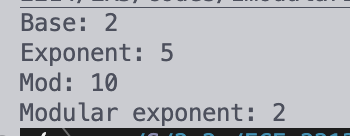
\includegraphics[width=.8\linewidth, height = .73in]{images/output/expo1.png}
        \caption*{}
        \label{fig:expo1}
    \end{subfigure}
    \begin{subfigure}{.5\textwidth}
        \centering
        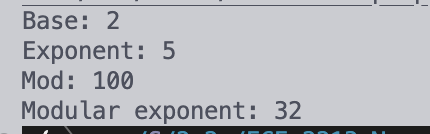
\includegraphics[width=.8\linewidth]{images/output/expo2.png}
        \caption*{}
        \label{fig:expo2}
    \end{subfigure}
    \begin{subfigure}{.5\textwidth}
        \centering
        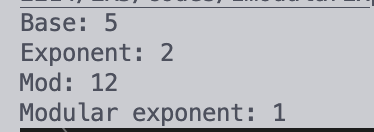
\includegraphics[width=.8\linewidth]{images/output/expo3.png}
        \caption*{}
        \label{fig:expo3}
    \end{subfigure}
    \begin{subfigure}{.5\textwidth}
        \centering
        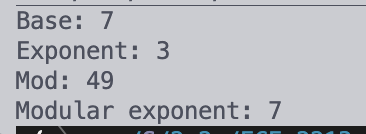
\includegraphics[width=.8\linewidth]{images/output/expo4.png}
        \caption*{}
        \label{fig:expo4}
    \end{subfigure}
    \caption{Outputs for Modular Exponentiation}
    \label{fig:expo}
\end{figure}
\begin{figure}[H]
    \begin{subfigure}{.5\textwidth}
        \centering
        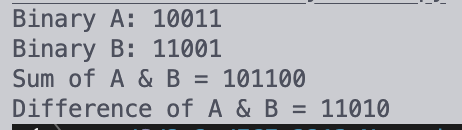
\includegraphics[width=.8\linewidth]{images/output/bin1.png}
        \caption*{}
        \label{fig:bin1}
    \end{subfigure}
    \begin{subfigure}{.5\textwidth}
        \centering
        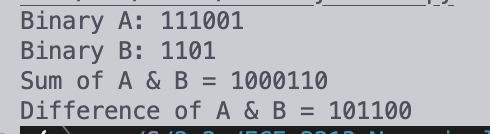
\includegraphics[width=.8\linewidth]{images/output/bin2.png}
        \caption*{}
        \label{fig:bin2}
    \end{subfigure}
    \newline
    \begin{subfigure}{.5\textwidth}
        \centering
        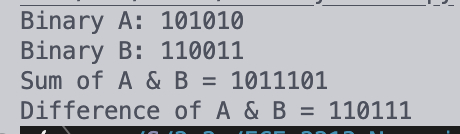
\includegraphics[width=.8\linewidth]{images/output/bin3.png}
        \caption*{}
        \label{fig:bin3}
    \end{subfigure}
    \begin{subfigure}{.5\textwidth}
        \centering
        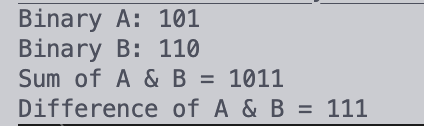
\includegraphics[width=.8\linewidth]{images/output/bin4.png}
        \caption*{}
        \label{fig:bin4}
    \end{subfigure}
    \caption{Outputs for Contraposition}
    \label{fig:bin}
\end{figure}

\begin{figure}[H]
    \begin{subfigure}{.5\textwidth}
        \centering
        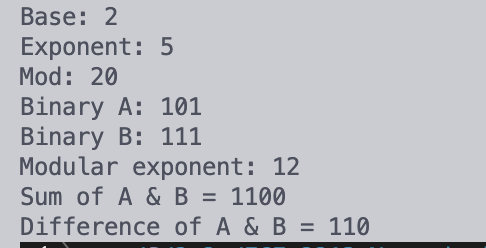
\includegraphics[width=.8\linewidth]{images/output/int1.png}
        \caption*{}
        \label{fig:int1}
    \end{subfigure}
    \begin{subfigure}{.5\textwidth}
        \centering
        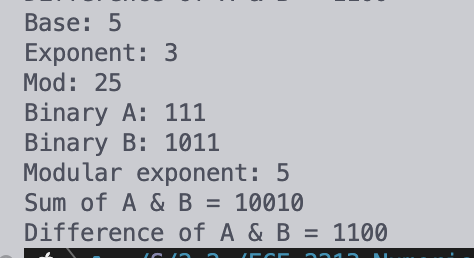
\includegraphics[width=.8\linewidth, height=1.1in]{images/output/int2.png}
        \caption*{}
        \label{fig:int2}
    \end{subfigure}
    \begin{subfigure}{.5\textwidth}
        \centering
        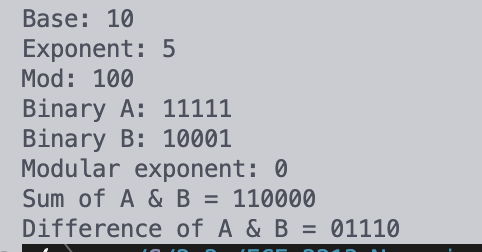
\includegraphics[width=.8\linewidth,]{images/output/int3.png}
        \caption*{}
        \label{fig:int3}
    \end{subfigure}
    \begin{subfigure}{.5\textwidth}
        \centering
        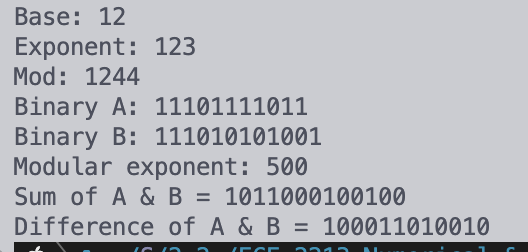
\includegraphics[width=.8\linewidth]{images/output/int4.png}
        \caption*{}
        \label{fig:int4}
    \end{subfigure}
    \caption{Outputs for Logical Equivalence}
    \label{fig:int}
\end{figure}


\section{Discussion}
To solve the three problems, the python library $Sympy$ was used. SymPy is an open source computer algebra system written in pure Python. It is built with a focus on extensibility and ease of use, through both interactive and programmatic applications.\cite{grangersympy} Using SymPy, the input logical sequence can easily be processed. otherwise there would be too many cases to take care of. Also it'll be harder to process big logical inputs.\\
Using SymPy's built-in functions, the inputs, which are logical sentences, are processed to a simplification, and then using other functions, the logical operations were done.


\bibliographystyle{APA}
\bibliography{ref}

\end{document}